This section is devoted to the investigation of the feedback structure that supports and shapes the system of automobility. \todonote{Perhaps this explanation of \emph{``why cars?''} could be in another chapter: methods? Introduction?}The choice of studying this particular transport mode is based on a triad of arguments: (a) the clear dominance of the automobile as the main mode of transport globally (in terms of travel demand), (b) the huge inertia, complexity and stability that the system has historically posed against threats to its dominance and (c) the fact that this dominance and resilience have become an obstacle for modal shifts, or more generally, a transition to sustainable mobility. Therefore, it is worth it to take a closer look at the dynamics that secure the position of automobility in its current status.

As an example of the automobility resilience, the system has ``survived'' the 1970s oil crisis, the ``dieselgate'' scandal\footnote{``Dieselgate'' refers to the Volkswagen emissions scandal that started in September 2015, when the U.S. Environmental Protection Agency reported that the German automotive industrial group had been faking emission control tests. This caused the \ce{NO_X} output to be lower in the certification tests than in real-world driving scenarios, thus being able to meet U.S. and European emission standards.} \parencite{guardian2017_Volkswagenrevealsrecord}, or even the 2008 global financial crisis. \fref{f:results:global-passenger-car-production} shows the global production of cars from 1961 to 2015, clearly depicting the effects of the financial crisis, whilst acknowledging that production has kept increasing nevertheless.
%
\begin{figure}[h]
\centering
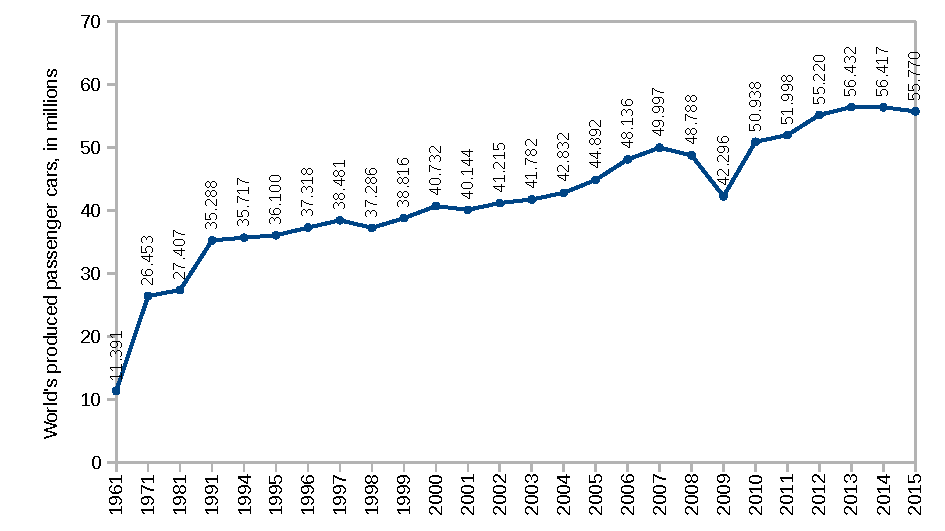
\includegraphics[width=0.85\textwidth]{figures/line_global-car-sales.pdf}
\caption[Global passenger cars production 1961-2015.]{Global passenger car production 1961-2015. Source: own figure; original data from \textcite{bts2017_Table123}.}
\label{f:results:global-passenger-car-production}
\end{figure}

As already mentioned in the \nameref{c:methods} chapter, the study of certain feedback structures of the system, detailed in the following subsections, is carried out through a series of Causal Loop Diagrams (CLD). Because of the resilient nature of the automobility regime, the collection of CLDs that form the overview of the system is referred to as the AUTOLOCK model. \ssref{ss:results:cld_urban-planning} discusses the stability mechanisms of automobility from an urban planning (land use) perspective. Next, the cultural basis and legitimacy apparatus of automobility is described in \ssref{ss:results:cld_cultural-feedbacks}.
% This section was removed Finally, \ssref{ss:results:cld_public-transport-automobility} provides a (partial) explanation of how automobility displaces public transport and vice-versa.

\textbf{Note:} with regards to notation: (a) CLD variables are denoted by a different font face, such as \CLDvar{This Example} and (b) causal loop (\emph{reinforcing} or \emph{balancing}) are denoted by the labels assigned in the diagrams, as in \CLDloop{R1}.

\todoparagraph{(OPTIONAL?)For each of the perspectives studied in the following subsections, a series of \glspl{PLP} are considered. This is, policy intervention is discussed on the basis of where in the feedback structure policy has the potential to be effective, avoiding policy resistance as much as possible.}

\subsection{Urban planning and automobility}
\label{ss:results:cld_urban-planning}
Historically, automobility is linked to the development of road infrastructure on one side and on cultural discourses that legitimise the adoption of private mobility on the other \parencite{goodwin2012_ProvidingRoadCapacity,gartman2004_ThreeAgesAutomobile,sheller2012_EmergenceNewCultures}. \fref{f:results:cld_congestion_1} shows the core reinforcing mechanism of automobility, which is founded on the mobility possibilities it supports, through increased \CLDvar{Accessibility} due to augmented \CLDvar{Road capacity}. Higher \CLDvar{Automobility demand} drives higher \CLDvar{Congestion}, putting pressure for more \CLDvar{Road investments}. \CLDvar{Accessibility}, coupled to a cultural background based on ideals of freedom, is seen as a major enabler for climbing up the social ladder, thus increasing \CLDvar{Automobile ownership} and closing the \CLDloop{R1} reinforcing loop --- the \emph{Automobility freedom} loop. With regards to the \CLDloop{R2} reinforcing loop, it accounts for a well-known rebound effect of motorway capacity expansion: induced travel demand \parencite{hymel2010_Induceddemandrebound,thill2005_Tripmakinginduced}. Most importantly, the cultural framework, represented by \CLDvar{Cultural legitimacy of automobility}, ultimately legitimises and supports these feedback structures.

\begin{figure}[h]
\centering
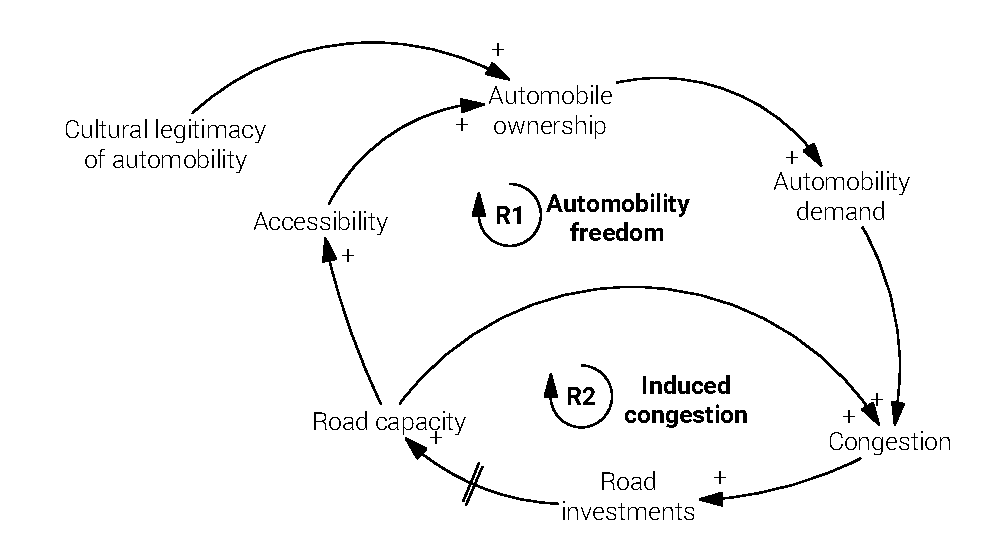
\includegraphics[width=0.7\textwidth]{figures/model/cropped/congestion-urban_1_core.pdf}
\caption{AUTOLOCK socio-spatial perspective: freedom and congestion.}
\label{f:results:cld_congestion_1}
\end{figure}

The increased accessibility provided by the ubiquitous construction (and expansion) of roads, coupled with low fuel/vehicle prices stirs the development of suburbs and causes a focus shift from the planning perspective, from integrated areas towards car-based single-use ones: the \CLDvar{Single-use urban development} variable in \fref{f:results:cld_congestion_2}. \CLDvar{Automobility demand} grows to meet the new requirements derived from the suburban lifestyle, namely the increase in spatial separation of jobs, housing, commercial and recreational areas; in other words, \CLDvar{Average travel distance}. Due to the low population density found in single-use urban developments, public transport becomes infeasible and expensive to maintain. Thus, the automobile rises as the single viable alternative for the residents of the suburbs, closing the \CLDloop{R3} reinforcing loop of \emph{automobility dependence}. This particular feature of the automobile system is particularly relevant for the focus of the present study. Automobility dependence locks in automobile users, planners, developers, etc. within the system practices space and forces them to adapt their lifestyles to this form of mobility \parencite{cullinane2003_Cardependencepublic,koehler2009_transitionsmodelsustainable}\footnote{The concept of \emph{practice space} is used by \textcite{koehler2009_transitionsmodelsustainable} to represent transport alternatives (including automobility) in their modelling and simulation of a sustainable transition.}.

Even though many cities worldwide have begun taking efforts to reduce automobile dependency (and have been doing so for years), it is critical to understand that the existing infrastructure, the huge sunk investments that have been brought into such infrastructure and the overall spatial organisation of residential, commercial and working areas has been built over many decades --- the inertia that these developments have is enormous \parencite{geels2012_AutomobilityTransitionSocio}. Not only because of the large amounts of resources that are needed to re-shape roads, cities and suburbs globally, but because the lifestyle that automobility is tied to has become deeply entrenched in cultural frameworks (as discussed in \sref{s:results:backcasting-ssp1-mob} and \ssref{ss:results:cld_cultural-feedbacks}).

\begin{figure}[h]
\centering
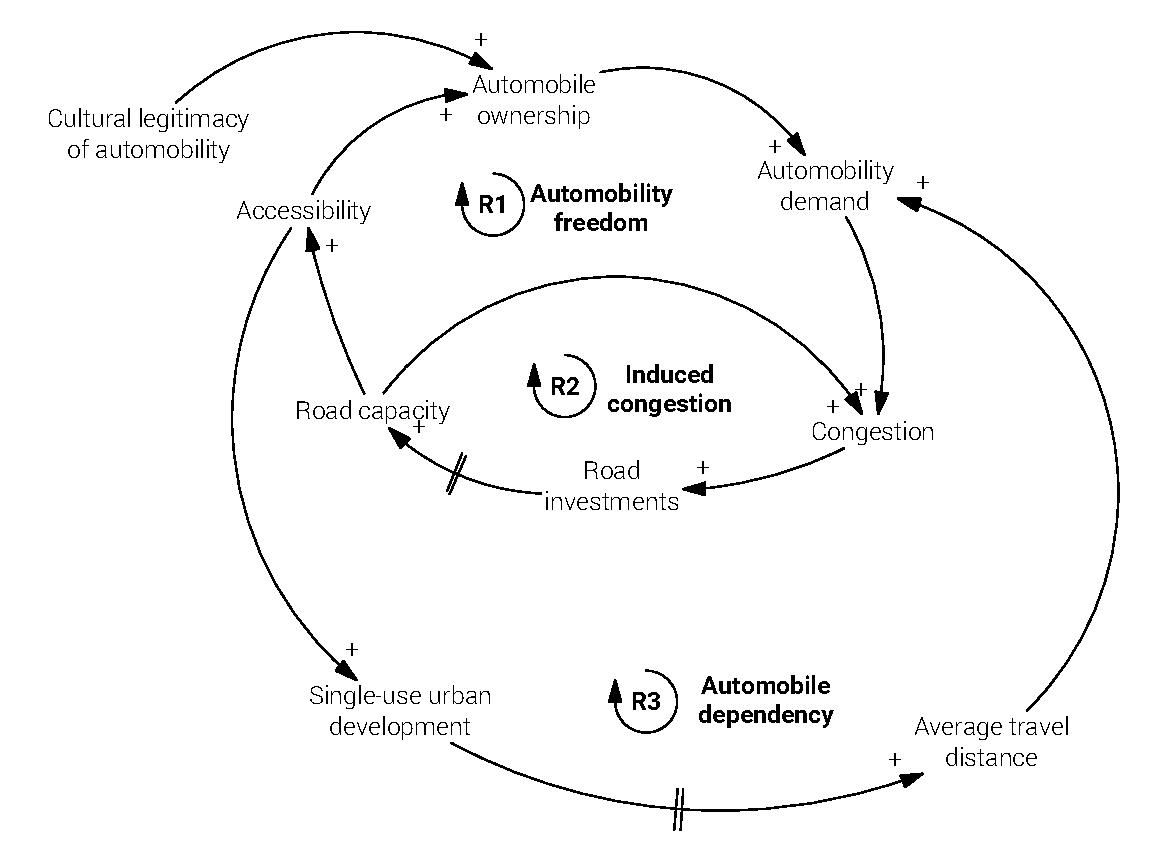
\includegraphics[width=0.8\textwidth]{figures/model/cropped/congestion-urban_2_dependency.pdf}
\caption{AUTOLOCK socio-spatial perspective: building automobile dependence.}
\label{f:results:cld_congestion_2}
\end{figure}

Finally, \fref{f:results:cld_congestion_3} presents additional balancing loops that restraint the further growth of mobility: some of them are endogenous, while some others (\CLDloop{B2} and \CLDloop{B3}) are exogenous\footnote{\emph{Endogenous} refers to dynamics arising from the inner-workings of the system or to actions to support it (single-use planning), while \emph{exogenous} refers to external measures/policies intended to counteract automobility use.}. For instance, \CLDvar{Average travel time} is an important factor contributing to the perceived accessibility that automobiles provide. If, due to congestion or longer travel distances, the time spent is excessive, the user might not find it convenient (accessible) to drive around. \CLDloop{B1} captures this phenomenon. When \CLDvar{Demand management policies} (e.g., road pricing) are introduced, another balancing feedback is produced, creating the \CLDloop{B2} loop \parencite{banister2008_sustainablemobilityparadigm,dudley2012_DynamicsRegimeStrength}.

Furthermore, the use of \CLDvar{Mixed-use urban development} techniques reduces, with time, the \CLDvar{Average travel distance}, thus alleviating the pressure on \CLDvar{Automobility demand}, portrayed in the \CLDloop{B3} balancing loop. However, the mutual exclusivity between mixed and single-use development patterns found in many regulatory frameworks \parencite{hirt2007_DevilIsDefinitions} means that they are in direct competition: if one planning practice increases, the other decreases and vice-versa. This feature is captured by the reinforcing loop \CLDloop{R5}. Finally, in a similar fashion to \CLDloop{B1}, another balancing force opposes the absolute dominance of automobiles: if suburbs grow in size and extension, not only time, but \CLDvar{Average travel distance} increases, thus reducing the perceived \CLDvar{Accessibility}, giving rise to \CLDloop{B4}.

\begin{figure}[h]
\centering
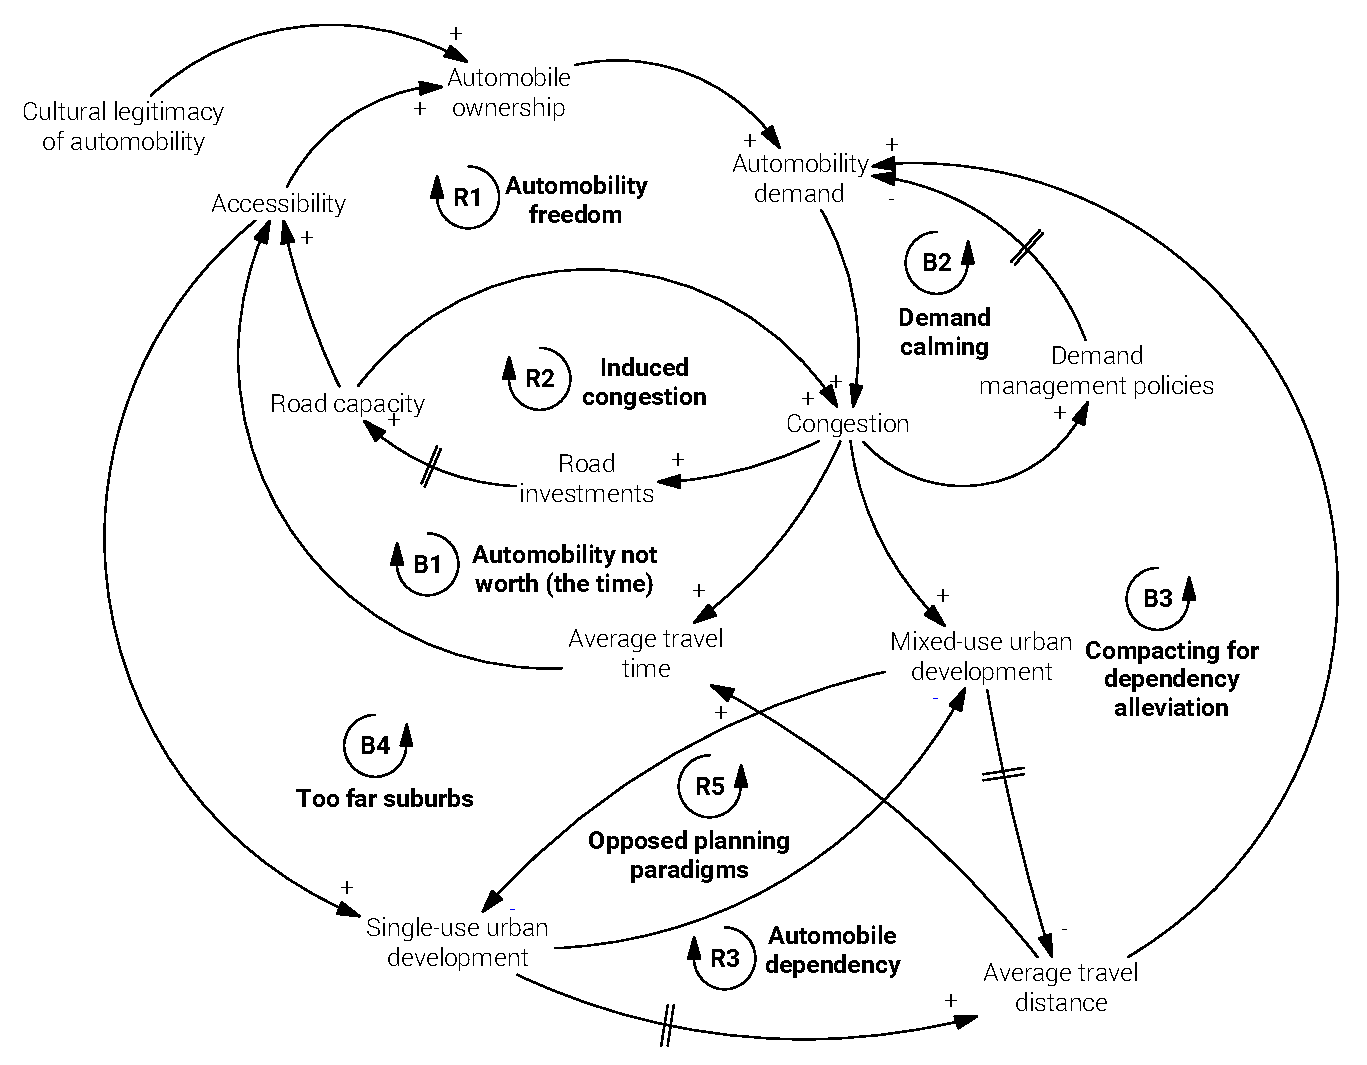
\includegraphics[width=\textwidth]{figures/model/cropped/congestion-urban_3_final.pdf}
\caption{AUTOLOCK socio-spatial perspective: balancing forces.}
\label{f:results:cld_congestion_3}
\end{figure}

\subsection{Cultural legitimacy feedbacks}
\label{ss:results:cld_cultural-feedbacks}
A highly relevant issue to discuss, with respect to the cultural dimension of automobility, is the legitimacy apparatus that supports it and, at the same time, dis-legitimises other forms of mobility (public transport, cycling, etc.). Due to the limitations in the scope of this study, only this central aspect will be analysed, since the range of practices and discourses that form the body of the automobility culture is huge. Therefore, this subsection is aimed at revealing the dynamics behind the \emph{acceptance} of automobility as a cultural reality.

\fref{f:results:cld_culture_1} draws from the CLD diagram in the previous section. The core reinforcing mechanism that drives \CLDvar{Automobility demand} growth (\CLDloop{R1}), is based on the \CLDvar{Cultural legitimacy of automobility}. However, unlike the CLD model in \ssref{ss:results:cld_urban-planning}, cultural legitimacy is not an external (supporting) force, but rather an integral part of the \emph{Freedom to move} discourse that sustains \CLDloop{R1}. The \CLDvar{Automobility capacity} variable is meant as the user's perception of the potential to access more destinations (accessibility) through better, uncongested roads (road capacity). Therefore, \CLDvar{Automobility capacity} is directly and proportionally linked to cultural legitimacy, since the perception of a higher ``degree of freedom'' reinforces the belief (the legitimacy) that automobility is the \emph{right} alternative to choose. However, there is a clear precondition that must hold to support this legitimacy dynamic: an framing \CLDvar{Discourse on individual freedom} as the highest (moral) value in the values hierarchy \parencite{urry2004_SystemAutomobility,boehm2006_PartOneConceptualizing,sheller2008_MobilityFreedomPublic}.

Secondly, \fref{f:results:cld_culture_1} shows another reinforcing loop, \CLDloop{R2}, that also contributes to increasing the \CLDvar{Cultural legitimacy of automobility}. It does so by providing the necessary lifestyle satisfaction (beyond the realisation of \emph{freedom}). Increased \CLDvar{Automobility capacity} enables the fulfilment of activities that (have) become embedded in the lifestyle: practices such as commuting, car-based grocery shopping, chauffeuring family members, weekend and holidays car-based tourism, etc. It is then important to understand that a lifestyle is a meaning carrier. Lifestyles are used to express one's identity, a ``narrative of the self''. Lifestyles are made of behaviours, conducts and practices that are adopted beyond their utility: they shape the individual's identity \parencite{giddens1991_ModernitySelfIdentity,spaargaren2000_Lifestylesconsumptionenvironment}. \CLDvar{Lifestyle satisfaction} then becomes the main mechanism to achieve a \CLDvar{Sense of individual identity} \parencite{ropke1999_dynamicswillingnessconsume}, closing the \CLDloop{R2} reinforcing loop, labelled as \emph{Seek for identity}.

\begin{figure}[h]
\centering
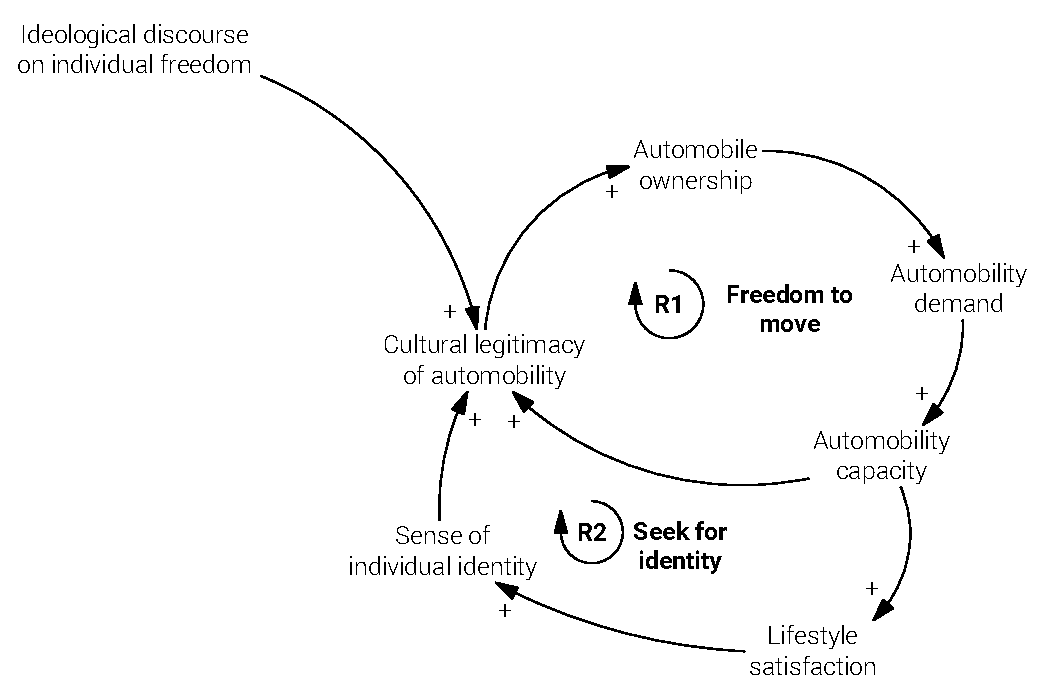
\includegraphics[width=0.7\textwidth]{figures/model/cropped/cultural_1_core.pdf}
\caption{AUTOLOCK cultural legitimacy perspective: identity and freedom.}
\label{f:results:cld_culture_1}
\end{figure}

\fref{f:results:cld_culture_2} adds an important feature of automobility: cultural homogenisation. \textcite{gartman2004_ThreeAgesAutomobile} argues that, similarly to other mass-manufactured products in the capitalist regime, automobiles have become yet another force of cultural homogenisation (\CLDvar{(Auto)mobility homogenisation}). This effect of the industrialisation of automobiles production, which holds especially during the Fordist era\footnote{Fordism refers to the application of manufacturing processes in the industry, following the example of Henry Ford. These techniques consist, in essence, of large-scale and highly mechanised production.}, leads to a decreased \CLDvar{Sense of individual identity}, since the ownership of an automobile no longer distinguishes an individual from another (everyone owns a car). This effectively closes a balancing loop, \CLDloop{B1}, where the loss of individuation power of automobility causes shrinking (or stagnant, at least) auto-ownership and demand.

As a response to the previous effect, the automotive industry has developed a new production pattern: a much wider range of automobile types (e.g., SUVs\footnote{SUV stands for \textit{S}port \textit{U}tility \textit{V}ehicle or \textit{S}uburban \textit{U}tility \textit{V}ehicle.}, hybrid cars, minivans, familiar vehicles, sportive cars, etc.) is offered to the users, with the intention to reach to lifestyle niches, that soon become mainstream markets on their own \parencite{gartman2004_ThreeAgesAutomobile}. This response proves to be effective, further accentuating the \CLDvar{Subcultural division} and, thus, satisfying the need for a \CLDvar{Sense of individual identity}. This mechanism is labelled in \fref{f:results:cld_culture_2} as the \CLDloop{R3} reinforcing loop of \emph{Cultural distinction}.

\begin{figure}[h]
\centering
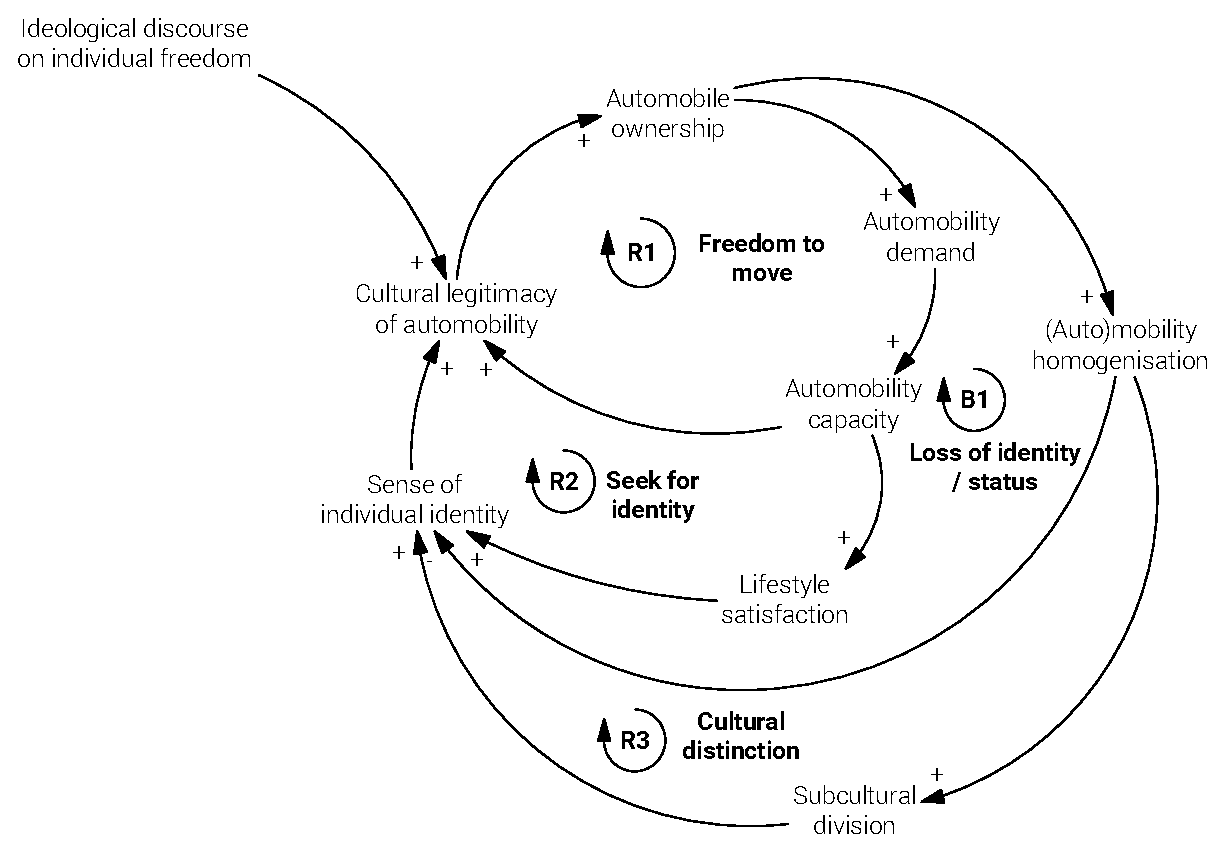
\includegraphics[width=\textwidth]{figures/model/cropped/cultural_2_subcultures.pdf}
\caption{AUTOLOCK cultural legitimacy perspective: homogenisation and subcultural division in (post)modernity.}
\label{f:results:cld_culture_2}
\end{figure}

\fref{f:results:cld_culture_3} incorporates a \emph{critical theory}\footnote{The \emph{critical theory} refers to the philosophical approach used by the scholars in the Frankfurt School to discuss issues such as the critique of capitalist societies, the modernities or the pursue of social emancipation.} approach to the analysis, investigating the origin of the \CLDvar{Need for individuation} that drives the legitimated institution of automobility as a integral component of the culture. The core of this analysis is the reinforcing loop \CLDloop{R4}, labelled \emph{Capitalism}, in which the concepts of \CLDvar{Socio-economic heteronomy}\footnote{\emph{Heteronomy}, in contrast to \emph{autonomy}, refers to the state in which an individual's actions are driven by forces external to itself. This is, heteronomous are those that are ruled by others. Note that, in the context of this study, the emphasis is put in the socio-economic aspect of heteronomy: the impossibility to conduct a lifestyle due to economic and social constraints (e.g., poverty, class conflicts, dominance/oppression relations, etc.).} and \CLDvar{Individual autonomy}\footnote{\emph{Autonomy} refers to the ability of an individual to be self-determined and self-governed.} are opposed. In the capitalist economy, class relations ultimately dictate the level of (socio-economic) autonomy an individual has. By not owning the production means, workers are highly heteronomous and bound to the forces of the labour market, social safety nets and other supra-individual institutions. In this context, due to the lack of \emph{political} \CLDvar{Individual autonomy}, identity is sought in \emph{cultural} individualisation (\CLDvar{Need for individuation}) \parencite{gartman2004_ThreeAgesAutomobile}.

\begin{figure}
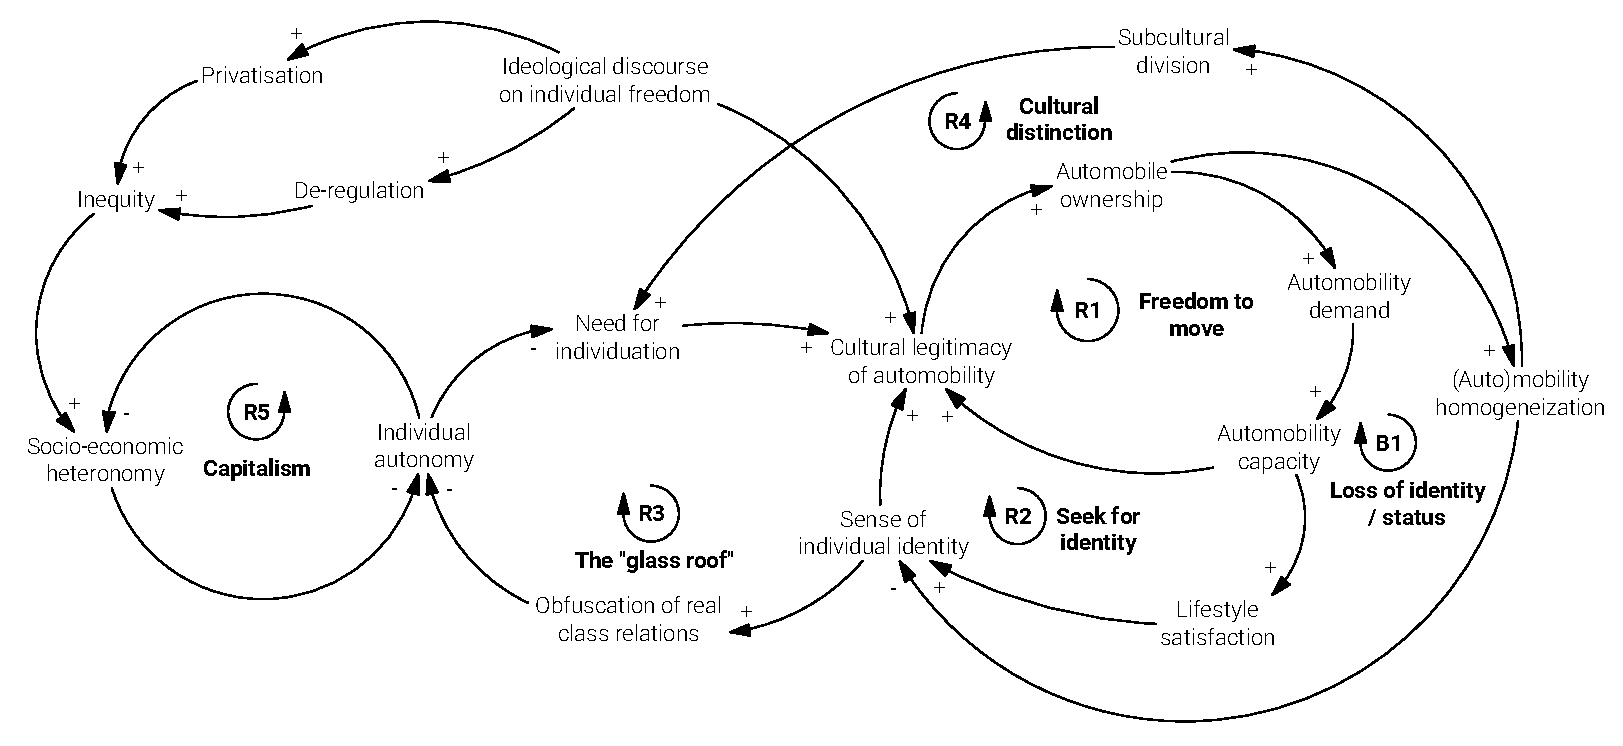
\includegraphics[width=1.2\textwidth,center]{figures/model/cropped/cultural_3_final.pdf}
\caption[AUTOLOCK cultural legitimacy perspective: class relations.]{AUTOLOCK cultural legitimacy perspective: class relations in neoliberal capitalism -- autonomy and heteronomy.}
\label{f:results:cld_culture_3}
\end{figure}

Further deep in the discussion about identity, individuality and autonomy/heteronomy, postmodernist\footnote{TODO} scholars claim that \CLDvar{Subcultural division} liberates individuals from class struggles. The liberation is due to the fact that identity is expressed within a subculture that is not necessarily superior to any other --- i.e., there is no hierarchy, no class \parencite{gartman2004_ThreeAgesAutomobile}. Under the postmodernist perspective, the automobile becomes a liberating product, with its capability to support many lifestyles.

However, the argument held by postmodernist scholars is a highly controversial one. Critical theory provides a very different explanation for the apparent relaxation of class conflicts in the late-capitalism era of mass consumption. The compensatory individuality sought in mass consumption (in automobility, in this study) to alleviate the deprivation of economic autonomy is not liberating. Instead, the mass consumption culture acts by hiding the real class relations: everyone, from all social classes, participates in the same consumption culture \parencite{gartman1991_CultureasClass,marcuse2013_OneDimensionalMan}. The boundaries of classes become diffuse in appearance and the (capitalist/automotive) culture becomes legitimised \parencite{gartman2004_ThreeAgesAutomobile}. These dynamics are presented in \fref{f:results:cld_culture_3} as the \CLDloop{R6} loop (\emph{The ``glass roof''}), which represents the hidden class relations that ultimately reinforce \CLDvar{Socio-economic heteronomy}. Also, the link from the \CLDvar{Need for individuation} variable to \CLDvar{Individual autonomy} is \emph{dashed}, to signify the postmodernist ``liberating'' individuality that subcultures produce, which is actually non-existent according to critical theory. 

Finally, a connection is depicted in \fref{f:results:cld_culture_3} from the overarching \CLDvar{Ideological discourse on individual freedom} to \CLDvar{Socio-economic heteronomy}, where (economic) \CLDvar{Inequity}, preceded by \CLDvar{Privatisation} and \CLDvar{De-regulation}, acts as the mediating mechanism. Following \textcite{monbiot2016_Neoliberalismideology,klein2008_shockdoctrinerise} analyses, the fundamentalist defence of unfettered (individual) freedom, comes at the expense of social/state interventions. The radical market ideology of neoliberalism is based on three tenets: \CLDvar{Privatisation}, \CLDvar{De-regulation} and free trade. It is now widely recognised that this ideology has brought huge increases in inequality during the last decades \parencite{milanovic2016_GlobalInequality,piketty2014_CapitalTwentyFirst}. Inequality is, precisely, the main source of \CLDvar{Socio-economic heteronomy}.

%\subsection{Public transport vs. Automobility}
%\label{ss:results:cld_public-transport-automobility}
%\todowarning{Is this section even necessary? What does it convey? Is there a way to incorporate stuff into the first CLD?}
%\begin{figure}[h]
%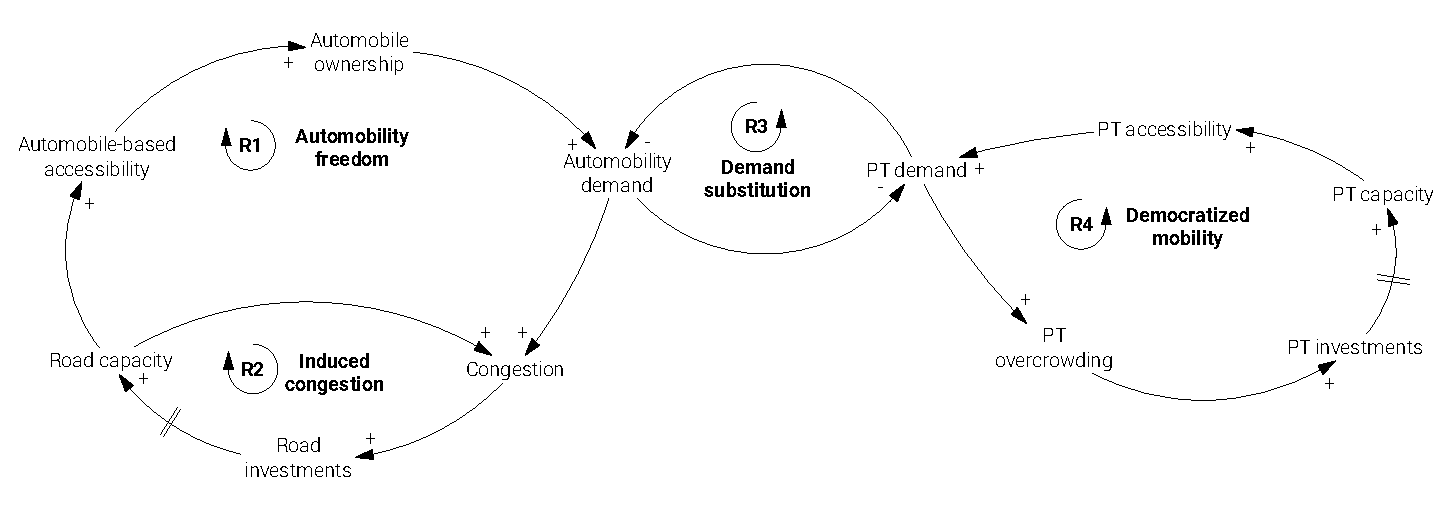
\includegraphics[width=1.1\textwidth,center]{figures/model/cropped/public-transport_1_core.pdf}
%\caption[]{}
%\label{f:results:cld_pt_1}
%\end{figure}
%
%\begin{figure}[h]
%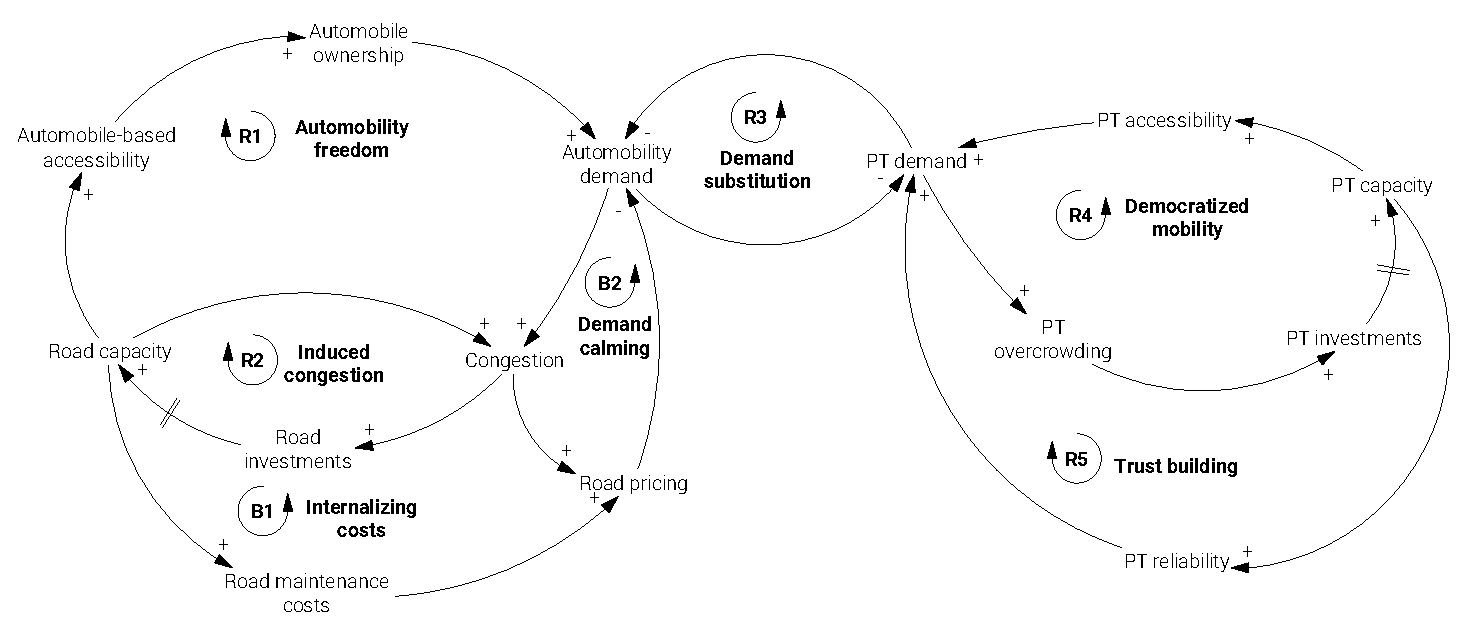
\includegraphics[width=1.1\textwidth,center]{figures/model/cropped/public-transport_2_trust.pdf}
%\caption[]{}
%\label{f:results:cld_pt_2}
%\end{figure}
%
%\begin{figure}
%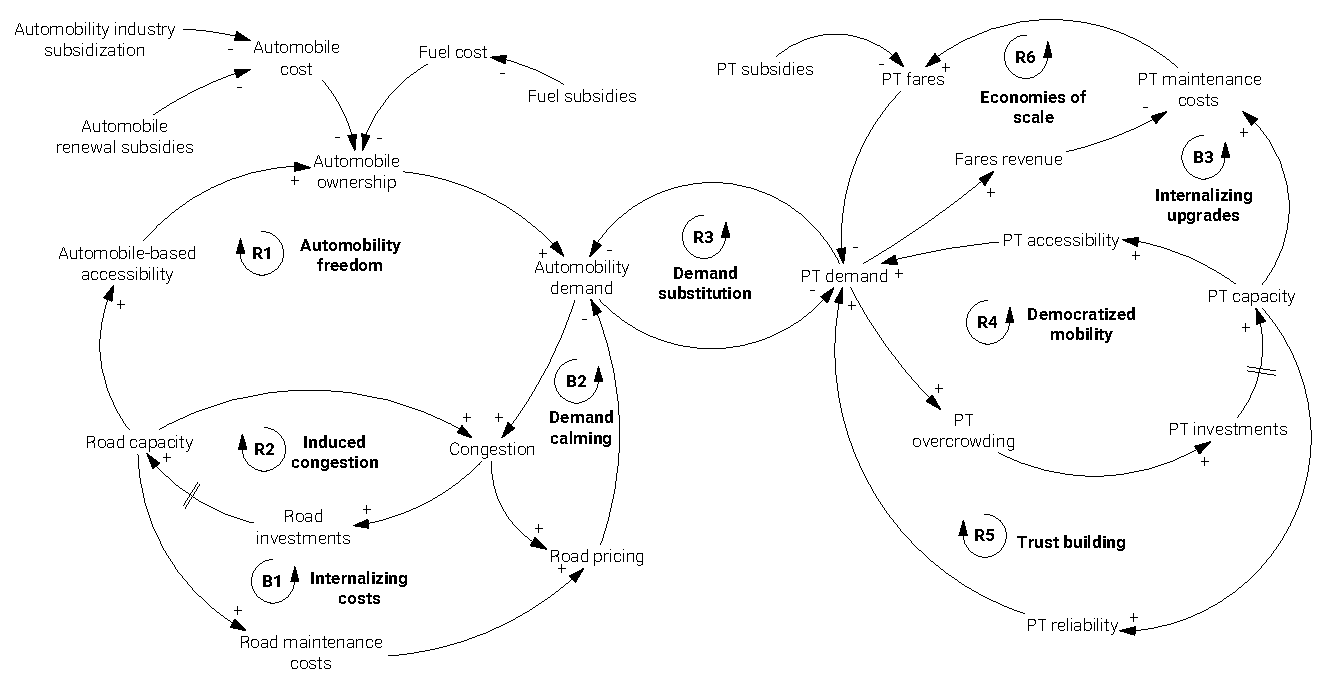
\includegraphics[width=1.2\textwidth,center]{figures/model/cropped/public-transport_3_final.pdf}
%\caption[]{}
%\label{f:results:cld_pt_3}
%\end{figure}